
\item
Esta gramática contiene un conflicto:

\begin{verbatim}
  %token D S

  %%
  p: ds ';' ss  | ss ;
  ds: D ';' ds    
    | D  
  ;
  ss: S ';' ss  | S  ;
  %% 
\end{verbatim}

\begin{itemize}
\item ¿En que consiste el conflicto?
\item
Reescriba la gramática para eliminar el conflicto
\end{itemize}


\item
\label{item:ambgrammar}
El siguiente lenguaje es intrínsecamente ambiguo y por tanto no puede ser completamente 
descrito por una gramática independiente del contexto:


 \[ \{ a^n b^n c^m : n \ge 0, m \ge 0 \} \cup \{ a^n b^m c^m : n \ge 0, m \ge 0 \} \]

Esto  es: Concatenaciones de repeticiones 
de $a$s seguidas de repeticiones de $b$s y seguidas de
repeticiones de $c$s donde el número
de $a$s es igual al número de $b$s
o bien el número de $b$s es igual al número de $c$s.

Escriba un programa Jison que reconozca este lenguaje.

\item 
Escriba un programa \verb|pegjs| que sin hacer uso de acciones semánticas
reconozca el lenguaje 
descrito en la pregunta
\ref{item:ambgrammar}.
Permita la presencia de blancos entre las letras \verb|a|, \verb|b| y \verb|c|.

\item 
Complete las partes de código que faltan 
en esta calculadora de expresiones aritméticas
escrita en pegjs-coffee:

\begin{verbatim}
{ 
  @reduce = (left, right)->  
    sum = left
    for t in right
      op = ____
      num = ____
      switch op 
        when '_' then __________
        when '_' then __________
        when '_' then __________
        when '_' then __________
        else _________________________
    sum
  
}
sum   = left:product _____:_______________ { @reduce(left, right); }
product = left:value _____:_____________   { @reduce(left, right); }
value   = number:[0-9]+                    { parseInt(number.join(''),10) }
        / '(' ____sum ')'                  { sum }
\end{verbatim}
\item 
Dada la gramática Jison:
\begin{verbatim}
A : A 'x' { $$ = do_x($1, $2); } | 'y' { $$ = do_y($1); }
\end{verbatim}
Encuentre un \verb|pegjs| que sea equivalente, tanto en el lenguaje reconocido como en 
la forma en que se ejecutan las acciones semánticas.


\item
Explique  en que consiste y como se lleva a cabo
el proceso de traducción realizado en la práctica de
clase {\it Calculadora con Análisis de Ámbito}
\ref{practica:ambitocalc}
desde el lenguaje fuente en el lado izquierdo
al lenguaje de una máquina
orientada a pila en el lado derecho.
Explique como funciona el acceso a las variables 
en lenguajes de programación que permiten 
ámbitos estáticamente anidados.

\begin{tabular}{|p{7cm}|p{7cm}|}
\hline
\begin{verbatim}
var c = 4, d = 1, e;
def g(a, b) { 
  var d, e; 
  def f(u, v) { a + u + v + d }
  a * f(b, 2) + d + c 
}
\end{verbatim}
&
\begin{verbatim}
        # global: var c,d,e
:g.f
        $a, 1
        $u, 0
        +
        $v, 0
        +
        d, 1
        +
        return
:g
        $a, 0
        $b, 0
        2
        call :g.f
        *
        d, 0     
        +
        c, 1
        +
        return
\end{verbatim}\\
\hline
\end{tabular}

Asegúrese de contestar a las preguntas que aparecen en la lista que sigue:
\begin{enumerate}
\item 
Dibuje el estado de la pila y los stack frames
en medio de la ejecución de \verb|f| cuando ha sido llamada 
desde \verb|g|.
%\begin{center}
%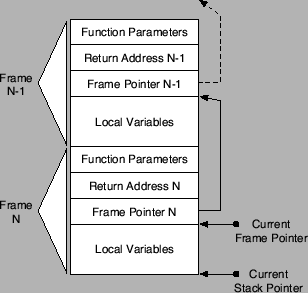
\includegraphics[width=0.7\linewidth]{stackframe.png}
%\end{center}

  ¿Donde se alojan los parámetros? ¿Y las variables locales? ¿Y la dirección de retorno?
  ¿Donde se aloja el enlace estático? ¿Que es el enlace estático?
  \item 
  ¿Que relación existe entre la forma en la que se guarden las variables y parámetros y la 
  presencia de recursividad en el lenguaje? ¿Como se relaciona esto mismo con la reentrancia?
  \item 
  En la llamada a un método en un lenguaje orientado a objetos 
  (por ejemplo C++), 
  ¿Donde se almacena la referencia al objeto actual asociado con el método?
\end{enumerate}


\item
La siguiente gramática no es LR(1).
\begin{verbatim}
[~/srcPLgrado/jison/jison-nolr]$ cat confusingsolvedppcr.y
%%
A: 
    B 'c' 'd' 
  | E 'c' 'f' 
;
B: 
    'x' 'y'
;
E: 
    'x' 'y' 
;

%%
\end{verbatim}
Encuentre una gramática Jison sin conflictos equivalente a la anterior.


\item
La siguiente gramática Jison presenta conflictos reduce-reduce:

\begin{verbatim}
[~/srcPLgrado/jison/jison-reducereduceconflict]$ cat reducereduceconflictPPCR2.y
%token ID

%%

def:    param_spec return_spec ','
        ;
param_spec:
             type
        |    name_list ':' type
        ;
return_spec:
             type
        |    name ':' type
        ;
type:        
             ID
        ;
name:        
             ID 
        ;
name_list:
             name
        |    name ',' name_list
        ;
%%
\end{verbatim}
Este es el diagnóstico de Jison:
\begin{verbatim}
~/srcPLgrado/jison/jison-reducereduceconflict]$ jison reducereduceconflictPPCR2.y
Conflict in grammar: multiple actions possible when lookahead token is ID in state 5
- reduce by rule: name -> ID
- reduce by rule: type -> ID
Conflict in grammar: multiple actions possible when lookahead token is : in state 5
- reduce by rule: name -> ID
- reduce by rule: type -> ID
Conflict in grammar: multiple actions possible when lookahead token is , in state 5
- reduce by rule: name -> ID
- reduce by rule: type -> ID

States with conflicts:
State 5
  type -> ID . #lookaheads= ID : ,
  name -> ID . #lookaheads= ID : ,
\end{verbatim}
Encuentre una gramática equivalente a la anterior sin conflictos.


\item
El lenguaje $\{ a^n b^n c^n / n \in \mathcal{N} \}$ no puede ser 
expresado mediante una gramática independiente del contexto.
Escriba un PEGJS (sin acciones semánticas)
que reconozca dicho lenguaje.
 
